\documentclass{article}
\usepackage[utf8]{inputenc}
\usepackage[spanish]{babel}
\usepackage{listings}
\usepackage{subfigure}
\usepackage{graphicx}
\usepackage{url}
\usepackage{multirow}
\usepackage{multicol}
\usepackage{color}
\usepackage{booktabs}
\usepackage{float}
\usepackage{amsmath,amssymb,amscd,amsthm}
%\usepackage{verbatim}
\usepackage{hyperref}
\hypersetup{
    colorlinks=true,
    linkcolor=blue,
    filecolor=magenta,      
    urlcolor=cyan,
}
\usepackage[margin=3cm,twoside]{geometry} 
\setlength{\parindent}{0pt}
\setlength{\parskip}{1em}
\usepackage{fancyvrb}
\usepackage{enumerate}
\newcommand\ql{\textquotedblleft}
\newcommand\qr{\textquotedblright}


\newcommand\E{\ensuremath{\mathbb{E}}}
\newcommand\N{\ensuremath{\mathbb{N}}}
\renewcommand{\P}{\ensuremath{\mathbb{P}}}
\newcommand\Q{\ensuremath{\mathbb{Q}}}
\newcommand\R{\ensuremath{\mathbb{R}}}
\newcommand\Z{\ensuremath{\mathbb{Z}}}

\newcommand\Om{\ensuremath{\Omega}}
\newcommand{\w}{\ensuremath{\omega}}

\newcommand\var[1]{\, \mathrm{Var} \left( #1 \right)}

\newcommand\pr[1]{\, \mathbb{P} \left( #1 \right)}

\newcommand\cov[1]{\, \mathrm{Cov} \left( #1 \right)}

\newcommand\espe[1]{\, \mathbb{E} \lbrack #1 \rbrack}



\definecolor{mygreen}{rgb}{0,0.6,0}
\definecolor{mygray}{rgb}{0.5,0.5,0.5}
\definecolor{mymauve}{rgb}{0.58,0,0.82}
\lstset{ 
  backgroundcolor=\color{white},   % choose the background color; you must add \usepackage{color} or \usepackage{xcolor}; should come as last argument
  basicstyle=\footnotesize,        % the size of the fonts that are used for the code
  breakatwhitespace=false,         % sets if automatic breaks should only happen at whitespace
  breaklines=true,                 % sets automatic line breaking
  captionpos=b,                    % sets the caption-position to bottom
  commentstyle=\color{mygreen},    % comment style
  deletekeywords={...},            % if you want to delete keywords from the given language
  escapeinside={\%*}{)},          % if you want to add LaTeX within your code
  extendedchars=true,              % lets you use non-ASCII characters; for 8-bits encodings only, does not work with UTF-8
  firstnumber=1,                % start line enumeration with line 1000
  frame=single,	                   % adds a frame around the code
  keepspaces=true,                 % keeps spaces in text, useful for keeping indentation of code (possibly needs columns=flexible)
  keywordstyle=\color{blue},       % keyword style
  language=Octave,                 % the language of the code
  morekeywords={*,...},            % if you want to add more keywords to the set
  numbers=left,                    % where to put the line-numbers; possible values are (none, left, right)
  numbersep=5pt,                   % how far the line-numbers are from the code
  numberstyle=\tiny\color{mygray}, % the style that is used for the line-numbers
  rulecolor=\color{black},         % if not set, the frame-color may be changed on line-breaks within not-black text (e.g. comments (green here))
  showspaces=false,                % show spaces everywhere adding particular underscores; it overrides 'showstringspaces'
  showstringspaces=false,          % underline spaces within strings only
  showtabs=false,                  % show tabs within strings adding particular underscores
  stepnumber=1,                    % the step between two line-numbers. If it's 1, each line will be numbered
  stringstyle=\color{mymauve},     % string literal style
  tabsize=2,	                   % sets default tabsize to 2 spaces
  title=\lstname                  % show the filename of files included with \lstinputlisting; also try caption instead of title
}
\usepackage{etoolbox}
\makeatletter
\providecommand{\subtitle}[1]{% add subtitle to \maketitle
  \apptocmd{\@title}{\par {\large #1 \par}}{}{}
}
\RecustomVerbatimCommand{\VerbatimInput}{VerbatimInput}%
{fontsize=\footnotesize,
	%
	frame=lines,  % top and bottom rule only
	framesep=2em, % separation between frame and text
	rulecolor=\color{mygreen},
	%
	label=\fbox{\color{black} prueba.txt},
	labelposition=topline,
	%
	commandchars=\|\(\), % escape character and argument delimiters for
	% commands within the verbatim
	%commentchar=*        % comment character
}
\renewcommand{\theenumi}{\roman{enumi}}
\newtheorem{teor}{Teorema}
\makeatother
 \title{Tarea 13 de Modelos Probabilistas Aplicados}
\subtitle{Teorema de límite central}
\author{5271}
\date{\today}

\begin{document}

\maketitle
\section{Introducción}
En este documento se presenta las nociones básicas sobre el teorema del limite central, ejemplos y aplicaciones.
\section{Teorema del limite central}
El teorema del límite central proporciona una aproximación al comportamiento de las sumas de variables aleatorias. El teorema establece que a medida que aumenta el número de variables aleatorias independientes e idénticamente distribuidas con media finita y varianza finita, la distribución de su suma se vuelve cada vez más normal independientemente de la forma de distribución de las variables aleatorias. Es decir, sea $X_1,X_2,...,X_n$ una secuencia de variables aleatorias mutuamente independientes e idénticamente distribuidas, cada una de las cuales tiene una media finita $\mu_{x}$ y una varianza finita $\sigma^{2}_{x}$. Sea $S_{n}$ definido como sigue:
\begin{align}
   S_n = X_1 + X_2 + \ldots + X_n. 
\end{align}
Ahora, $\espe{S_n}= n\mu_{x}$ y $\sigma^{2}_{S_{n}}= n\sigma^{2}_{x}$ . Al convertir $S_n$ en una variable aleatoria normal estándar (es decir, media cero y varianza unitaria), se obtiene.

\begin{align}
    Y_n = \dfrac{S_n-\espe{S_n}}{\sigma^{2}_{S_{n}}}= \dfrac{S_n-n\mu_{X}}{\sigma_X\sqrt{n}}.
\end{align}
El teorema del límite central establece que si $F_{Y_{n}}(y)$ es la función de densidad  de $\gamma_n$ , entonces:
\begin{equation}
	\lim_{n \rightarrow \infty} F_{Y_{n}}(y) =\lim_{n \rightarrow \infty} \P{\left[Y_{n}\leq y \right]} = \int_{-\infty}^{y} \frac{1}{\sqrt{2 \pi}} e^{-u^2 / 2} \, du = \Phi(y) ;
\end{equation}
Esto significa que $\lim_{n \rightarrow \infty}\gamma_{n}$ se distribuye $\sim N(0,1)$. Por tanto, uno de los roles importantes que juega la distribución normal en estadística es su utilidad como aproximación de otras funciones de distribución de probabilidad.
Lo anterior se apoya en el teorema 9.5 del libro ``\textit{Introduction to Probability}''\cite{libProba}:


 Para una mejor comprensión de lo anteriormente expuesto se tomará como ejemplo la resolución del ejercicio 11 de la página 355 del mismo libro, que dice:
 
\textit{A tourist in Las Vegas was attracted by a certain gambling game in which the customer stakes 1 dollar on each play; a win then pays the customer 2 dollars plus the return of her stake, although a loss costs her only her stake.Las Vegas insiders, and alert students of probability theory, know that the probability of winning at this game is 1/4. When driven from the tables by hunger, the tourist had played this game 240 times. Assuming that no near miracles happened, about how much poorer was the tourist upon leaving the casino? What is the probability that she lost no money?
} 

Para resolver este ejercicio se realiza el programa \ref{cod:1} en lenguaje R \cite{R} que se muestra a continuación.

\begin{center}
\lstinputlisting[ language=R, firstline=1, lastline=17]{Tarea14.R}
\label{cod:1}
\end{center}
 Como respuesta a la primera pregunta se tiene que $\espe{S_n}= n\mu_{x}=-60$, por lo que si el turista juega 240 veces se espera que pierda 60 dolares. Para la segunda respuesta tenemos la figura \ref{fig:1} de la página \pageref{fig:1}, que muestra una simulación de 240 veces jugadas con una distribución normal con media $\mu= -60$ y $\sigma^{2} = 6.708$. en la misma se puede observar que existe cero probabilidad que el jugador gane algún dolar en un total de 240 juegos.  
 \vspace{-0.5cm}
\begin{figure}
    \centering
    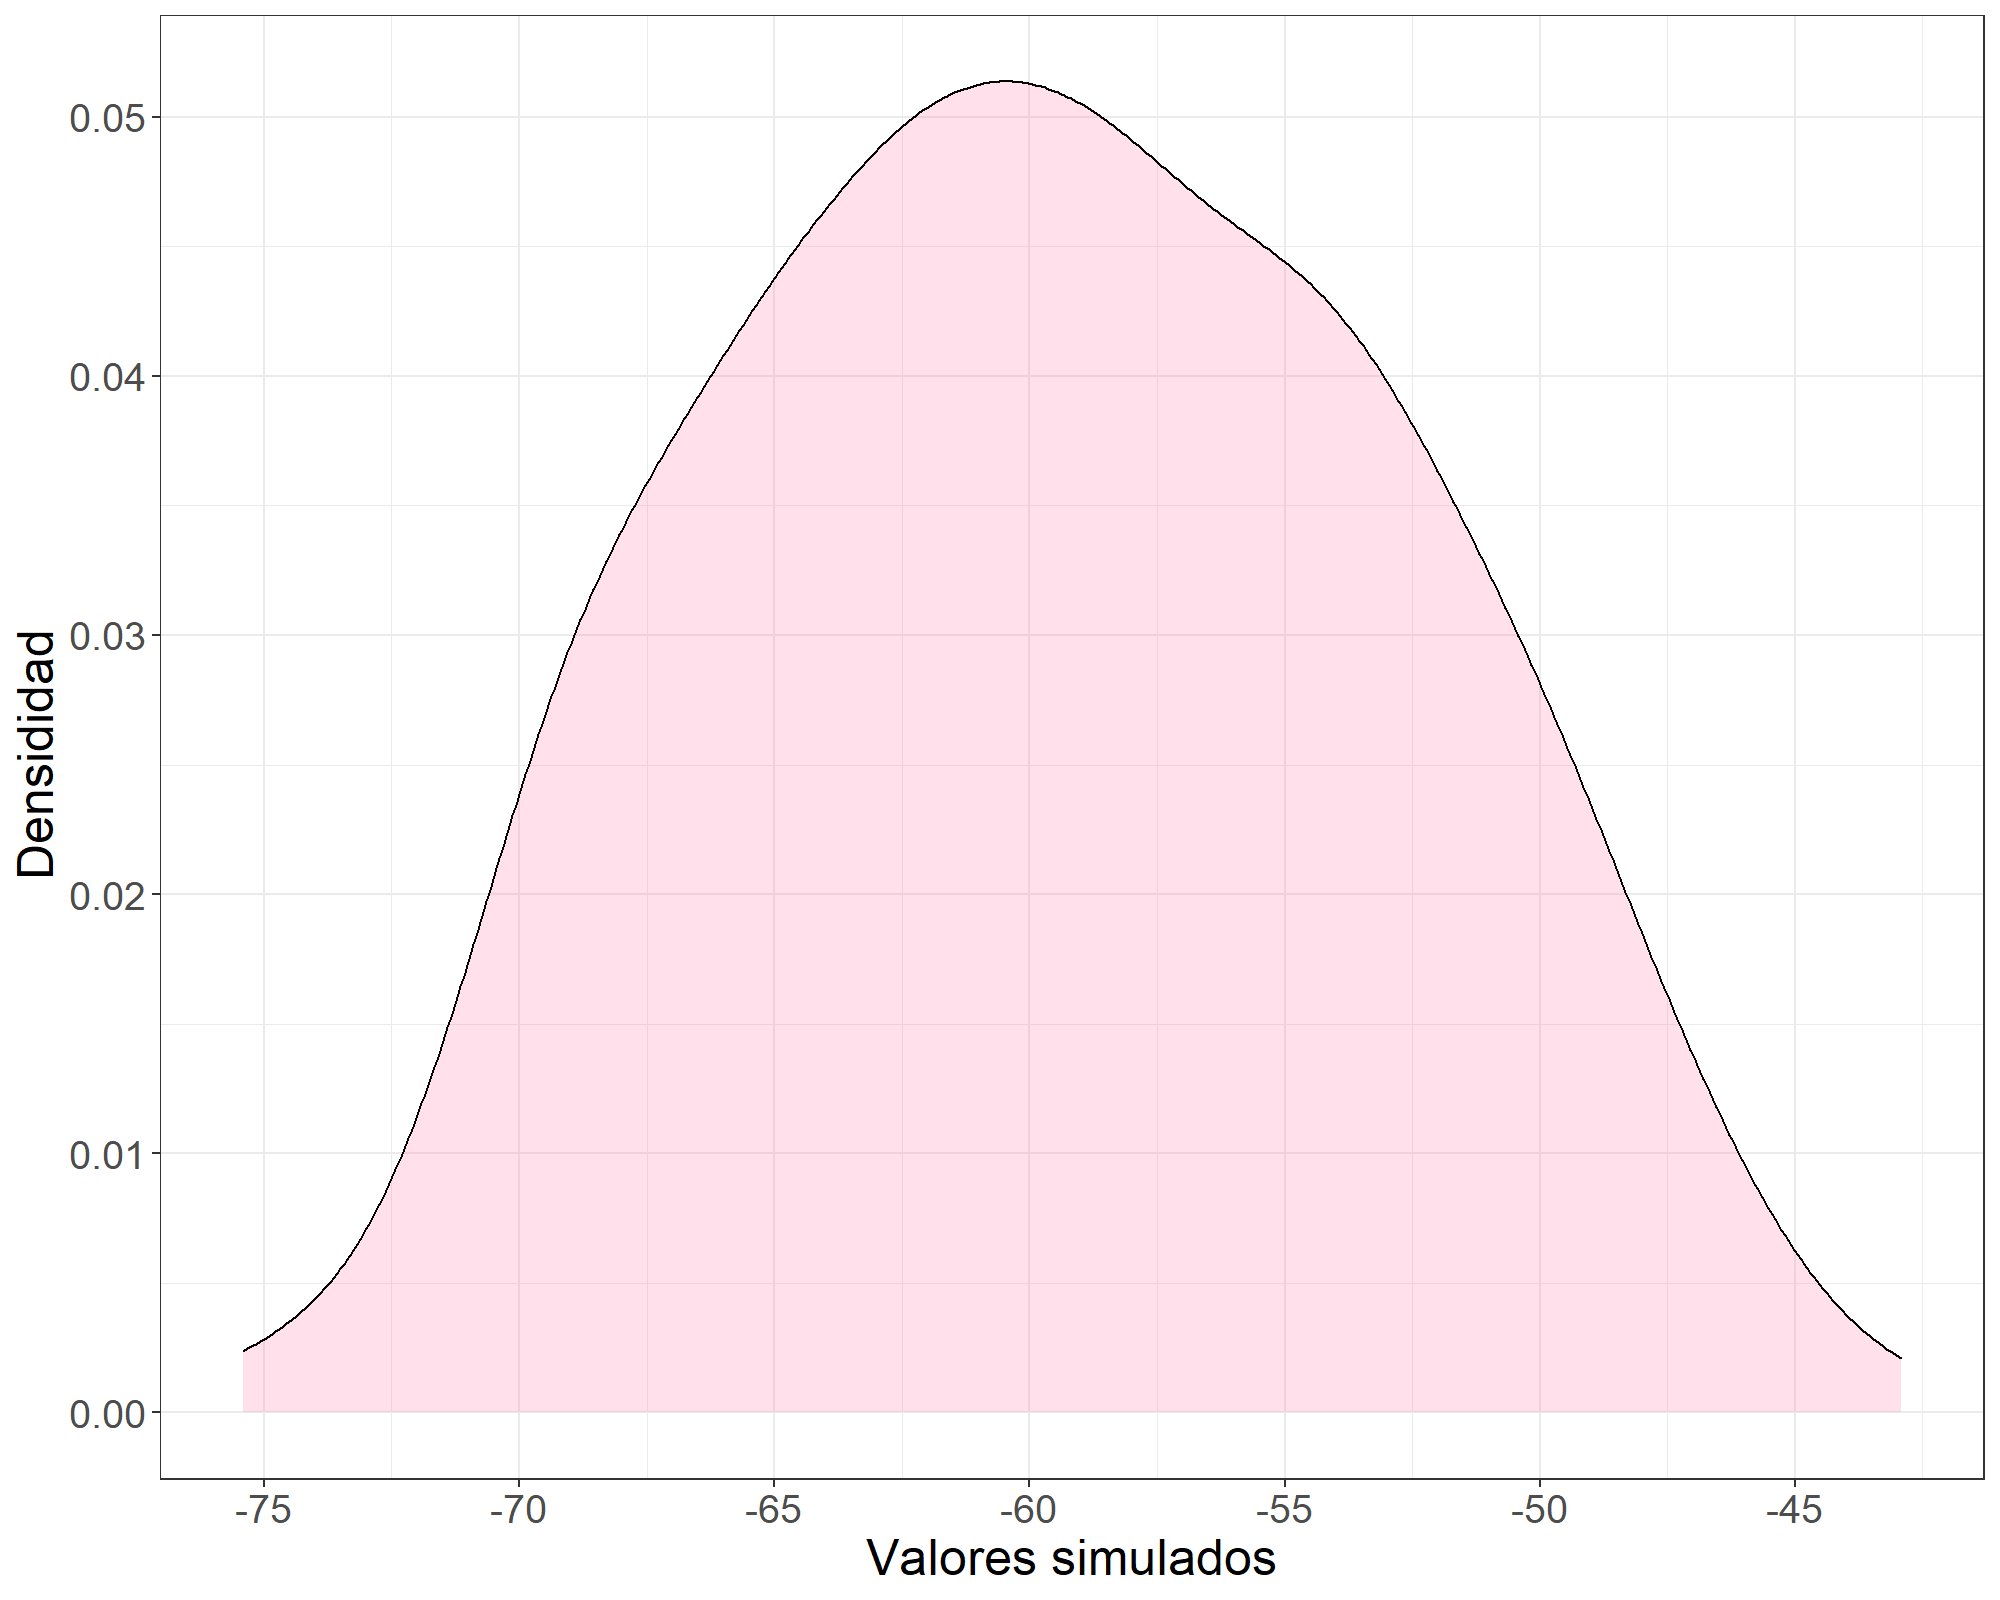
\includegraphics[scale=0.35]{figuras/ejercicio11.png}
    \caption{Diagrama de densidad de los resultados para 100 repeticiones del experimento.}
    \label{fig:1}
\end{figure}
\section{Aplicación en prueba de hipótesis } 
En esta sección un ejemplo de como se utiliza el teorema del limite central para probar hipótesis. Comúnmente para esta fin se utiliza una prueba de $\chi^2$  para determinar si rechazar una distribución de población hipotética (con un número finito de clases)como falso. Aquí se hará esto para cuando la población se descomponga en dos clases (fumadores y no fumadores).

Para el ejemplo plantearemos la hipótesis $H_0$ que nos dice que el 20 \% de los jóvenes en Monterrey fuman, para probar esta hipótesis tomamos datos de una encuesta realizada a 1,888 estudiantes en Monterrey \cite{encu} la cual arroja que 18.7 \% de los encuestados eran fumadores al momento de la realización de la encuesta.

Sea $X_i = 1$ si el encuestado $i$ dice que es fumador, y sea $X_i = 0$ si el encuestado $i$ dice que no es fumador. Estas $X_i$ son variables aleatorias de Bernoulli independientes. Tenemos que $S_n = X 1 + ··· + X_1,888$. Si la hipótesis de que el 20\% de los jóvenes de Monterrey fuman es correcta, entonces $\mu = \espe{X_i} = 0.2$, y $\Var {X_i} = µ (1 - µ) = 0.16$; y entonces, el teorema del límite central nos diría que:
\begin{align}\label{eq:1}
   \frac{S_{1888}-378}{\sqrt{1,888 \cdot 0.16}}, 
\end{align}
 en el sentido que
\begin{align}
    \P \left( \frac{S_{1888}-378}{6.952} \leq y \right)\approx \Phi(y).
\end{align}
Ahora, si $S^{*}_{1,888}$ es el valor observado $S_{1,888}^1$, y si
    \begin{align}\label{eq:2}
  \gamma= \frac{S_{1888}-378}{\sqrt{6.952}}, 
\end{align}    
entonces, sobre la base del teorema del limite central y la ecuación \reef{eq:1} se esperaría que $\gamma$ es un valor atípico para $\sim N(0,1)$. Específicamente, no se esperaría que $\gamma$ demasiado grande; es decir no se esperaría que:
\begin{align}
    \P (|N(0,1)|\gep |\gamma|)<0.05,
\end{align}
  si $\mu=0.2$ es la media verdadera.
Así se tiene la siguiente prueba estadística: Se fija un $\alpha >0$, comúnmente se emplea $\alpha =0.05$. Calculando $\gamma$ como en la ecuación \ref{eq:2}, si
\begin{align}
    \P  (|N(0,1)|\gep |\gamma|)= 2\Phi(-|\gamma|)<\alpha,
\end{align}
rechazamos la hipótesis de que el valor medio de $X_i$ es $\mu$, y si esta desigualdad no se satisface, no la rechazamos.

Por lo que se tiene que:

\begin{equation}
    \gamma = \frac{353-378}{6.952}= -3.596,
  \end{equation}
    y calculando vemos clara mente que
   \begin{equation}
    2\Phi(-3.596)= 2(0.49983)= 0.9996>0.05.
  \end{equation}
  Por lo tanto no hay suficientes elementos para rechazar $H_o$, que plantea que el 20\% de los jóvenes en Monterrey fuman. $H_0$ se acepta con un intervalo de confianza del 95\%.
\newpage
\bibliographystyle{plain}
\bibliography{Biblio}

\end{document}

